\scanpage{11}
\uline{Exemple} \quad $A$ anneau \unsure{C|(}

$f\in A$ élément régulier

$g\in A$ élément $(A/fA)$\inserted{$=B$}-régulier, \unsure{\&}

on suppose $A/fA+gA\ne0$ i.e. $B/gB\ne0$

[On peut supposer $A$ noethérien régulier de dim $2$,
$A/fA$ noeth. régulier de dim $1$,
$A/fA+gA$ noeth. \unsure{régulier|artinien} de dim $0$,
p.ex $A$ anneau local régulier de dim $2$,
$(f,g)$ système de paramètres]

On va construire un module $M$ sur $A$ tel que
\[
\text{(i)}\quad M=\bigcup_{n\geq0}{}_{f^n}M,\qquad
{}_{f^{n+1}}M/{}_{f^{\unsure{n+n|n}}}M\simeq A/fA
\]
[en particulier, $M$ est de support $\subset V(f)$ et est
$fA$-\unsure{cofini}]
\[
\text{(ii)}\quad M/fM\simeq(A/fA+gA)^{(\unsure{\mathbb N|\mathbf N})}\inserted{=(B/gB)^{(\unsure{\mathbb N|\mathbf N})}}
\]
donc $M/fM$ n'est pas $fA$-cofini.

\uline{Construction}. On construit par récurrence les
${}_{f^n}M$ comme $E_n$, l'hypothèse de
récurrence étant
\[
\left\{\begin{aligned}
\text{(a)}_n\quad & f^nE_n=0\\
\text{(b)}_n\quad & {}_{f^{k+1}}E_n/{}_{f^k}E_n\simeq A/fA=B\qquad(0\leq k\leq n-1)\\
\text{(c)}\quad & E_n/fE_n\simeq\deleted{\unsure{A/fA}}B+(B/gB)^{n-1}
\end{aligned}\right.
\]
\mspage{10}
\margin{\figure{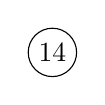
\begin{tikzpicture}[baseline=(n.base)]\node[draw,circle,inner sep=2pt] (n) {\unsure{14}};\end{tikzpicture}}}

